\documentclass[11pt, oneside]{article}   	
\usepackage{geometry}                		
\geometry{letterpaper, margin=1in}              
\usepackage{graphicx}					
\usepackage{amssymb}
\usepackage{amsmath}
\usepackage{booktabs}
\usepackage{listings}
\usepackage{color}
\usepackage{multirow}

\definecolor{dkgreen}{rgb}{0,0.6,0}
\definecolor{gray}{rgb}{0.5,0.5,0.5}
\definecolor{mauve}{rgb}{0.58,0,0.82}

\lstset{frame=tb,
   language=[90]Fortran,
   aboveskip=3mm,
   belowskip=3mm,
   showstringspaces=false,
   columns=flexible,
   basicstyle={\small\ttfamily},
   numbers=none,
   numberstyle=\tiny\color{gray},
   keywordstyle=\color{blue},
   commentstyle=\color{dkgreen},
   stringstyle=\color{mauve},
   breaklines=true,
   breakatwhitespace=true
   tabsize=3
   }


\title{MCSC 6030G : High Performance Computing \\ Assignment 2: Langevin Dynamics}
\author{Parikshit Bajpai \\ 100693928}
\date{}							% Activate to display a given date or no date

\begin{document}
\maketitle

\section{Introduction}
In 1908, Paul Langevin successfully applied Newtonian dynamics to a Brownian particle to come up with what is now called as the 'Langevin equation', the stochastic physics equivalent to the second law of motion (\(F=ma\)). This stochastic differential equation is applicable to continous Markov processes and shows that the root mean square dispalcement of a Brownian particle is proportional to the square root of time. The Langevin equation contains both viscous and random forces with the two forces related by the  fluctuation-dissipation theorem. In the modern notation, Langevin equation takes the following form:     
  \begin{equation} \label{Langevin}
    m\,dv = - \gamma\,v\,dt + \sqrt{dt}\,c\,\eta(t) 
  \end{equation}
where the velocity of the particle, \(v \in \in^2\) in a two-dimensional space, \(\gamma\)  denotes the viscosity contribution of the force, and the random force variable \(\eta\) is drawn from a standard normal distribution. The random force  coefficient equals, from the fluctuation-dissipation theorem, \(c = \sqrt{2 \gamma k_B T}\), where \(k_B\) is the Boltzmann constant and T is the temperature.  

\section{Methodology}
\subsection{Objective}
The objective of this study is to analyze the non-interacting particle Brownian motion and analyze the simlifying assumptions adopted in the implementation, assess the requirements for parallelization and study their implementation, and to develop test cases to verify the implementation. 

\subsection{Machine Configuration}
	\textbf{Manufacturer \& Model}: Lenovo ThinkPad Yoga 370\\
	\textbf{Processor}: Intel Core i5 -7200U (4 processor cores)\\
	\textbf{Clock Rate}:  2.50 GHz\\
	\textbf{RAM}:  16 GB\\
	\textbf{Operating System}: Ubuntu 18.04\\
	

Marcos Machado, Celina Desbiens and myself worked together on building the codes, executing and interpreting the results. 
	
\section{Results and Discussion}
\textbf{(1)}\quad The mass, space and time scales can be defined for the  Langevin equation in terms of the system parameters as follows: \[Mass scale [s] = m\]  \[Time scale [s] = \frac{m}{\gamma}\]  \[Space scale [s] = \frac{\sqrt{m}\cdot c}{\sqrt{\gamma^3}}\]

Since, for the purpose of numerical approximation, \(m\) and \(k_B T\) play the role in scaling and do not affect the nature of the stochastic equation, we can set them both equal to 1 in the code. This does not affect the behaviour that we want to observe which relates to the time scale.

The additional dimensionless parameter when considering a closed box of dimension \(L \times L\) arises from the \(\gamma\) term which inherently contains a length scale related to the radius of the Brownian particles and when the domain gets contrained, the factor L alongwith \(\gamma\) results in a new dimensionless constant.


\textbf{(2)}\quad Parallelisation was implemented using OpenMP directives and we observe a change in the structure of the code in order to reap the maximum benefits of parallelisation. In the present case, two threads were used with one thread handling the computation and the other thread handling the writing to disk. This was done since writing is the most time consuming process in the code and with the vectorized code implementation, the computational time is no more a stumbling block in the performance. In order to implement the  parallelisation, we must ensure that the race condition must not arise. With this aim, the time variable, \textit{t}, was listed using the \textit{lastprivate} \& \textit{lastprivate} clauses and temporary variables \textit{x\_temp} \& \textit{y\_temp} were defined. Moreover, since writing and computing are now handled by separate threads, the writing task does not necessarily need to follow the computation. In fact, we see from the code that the OpenMP section responsible for writing data to disk precedes the OpenMP section looping over the particles to run the velocity verlet algorithm.

A direct comparison of the two codes can be performed in terms of the speed-up. The obtained results have been presented in  table~\ref{tab:su}
\begin{table}[h]
  \caption{Speed-up and efficiency of parallelisation.}
  \label{tab:su}
  \centering
  \begin{tabular}{lcrrcrr}
    \toprule
    \multirow{2}{*}{Optimization} &\phantom{abc} & \multicolumn{2}{c}{Wall Time [s]} &\phantom{abc} & \multicolumn{2}{c}{Parameter} \\
    \cmidrule{3-4} \cmidrule{6-7}
    &\phantom{abc} & {Serial} & {Parallel} & \phantom{abc} & {Speed-up} & {Efficiency}\\
    \midrule
    O0 && 0 & 0 && 0 & 0\\
    O3 && 0 & 0 && 0 & 0\\
    \bottomrule
  \end{tabular}
\end{table}

\textbf{(3)}\quad (a) One of the possible tests to verify the particle distribution is to divide the box into sectors and count the number of particles in each sector. Since the particles have been distributed uniformally, all the boxes should contain almost the same number of particles.\\
(b) Another possible test to check the proper implementation of the boundary conditions is to count the total number of particles in the box at \(t_0\) and \(T_{max}\). Provided that the particles have reasonable velocities and accelarations, the number of particles lost during the simulation must be reasonably small.\\ (c) The root mean square displacement of the particles should show two distinct phase - a ballistic phase with root mean square dispacement proportional to \(t\) and a Brownian motion phase with root mean square displacement proportional to \(t^{1/2}\). Furthermore, when a box of sufficiently large dimensions is used, the root mean square displacement should reach a constant plateau after a the ballistic and Brownian phases.     

\textbf{(4)}\quad The velocity autocorrelation function can be defined as \[A(\tau) = \frac{\langle v(t) \cdot v(t-\tau)}{\langle v(t) \cdot v(t)}\] From the requirement of equipartition of energy at equilibrium, it can be shown that the autocorrelation function, \(A(\tau)\) decays as \(\exp{-\gamma t / m}\). To observe this behaviour, the following implementaion of the autocorrelation function was implemented: \[A(t) = \frac{\langle v(t) \cdot v(0)}{\langle v(t) \cdot v(t)}\] This implementation of the velocity correlation function was implemented using the following additional lines of code:

\begin{lstlisting}
  ! Declare variables to save initial velocity for correlation
  double precision, allocatable, dimension(:) :: vx0,vy0
  .
  .
  ! In the subroutine initialize\_particles, save the initial velocities in vx0 and vy0
  vx0(i)=vx(i)
  vy0(i)=vy(i)
  .
  .
  ! Open additional file to save the velocity correlation function
  open(13,file='velocity_correlation')
  .
  .
  .
  do while(t.lt.t_max)
     .
     .
     write(13,*) t,(sum(vx*vx0 + vy*vy0)/real(n,8))/(sum(vx*vx + vy*vy)/real(n,8))
  end do
\end{lstlisting}     

The additional line in the code writes the velocity correlation at each time step to the file \textit{velocity\_correlation} and the values were plotted against time. As shown in figure~\ref{fig:vcf}, the velocity correlation function follows the desired exponentially decaying trend but the exact values shows a slight departure from the exact expected curve. This fluctutaion is a result of the statistical nature of the function and the trend confirms the expected behaviour. 
	\begin{figure}[h]
		\centering
		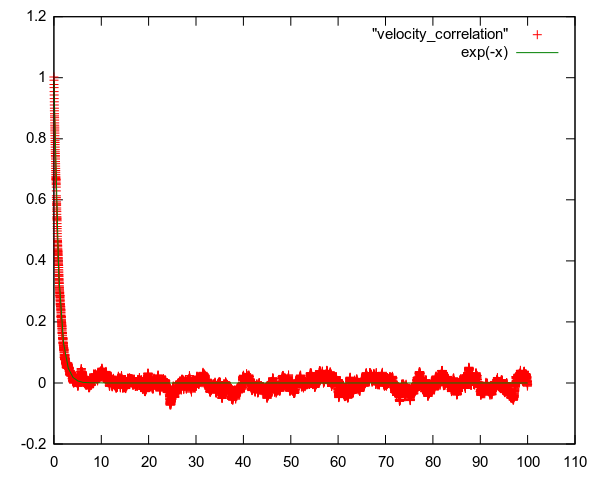
\includegraphics[width=\textwidth]{vcf.png}
		\caption{Computed velocity correlation function and expected behaviour.}
		\label{fig:vcf}
	\end{figure} 


        However, we also notice that the speed up did not increase linearly when the number of threads was increased from 2 to 4. Such a non-linear increase can, most probably, be attributed to increase in overheads as the number of threads is increased. Use of the BLAS library with \textit{gfortran} compiler resulted in the most significant increase in speed up. However, the wall times using OpenMP and BLAS concurrently were higher than the wall times obtained using them individually. For the sake of brevity, these results, therefore, have not been presented. They can, however, be viewed by running the shell script \textit{run.sh} in the repository.

 

\section{Conclusion}
In the present exercise, the impact of parallelisation on the code was analysed using speed-up and efficiency and a number of test cases were developed. It was observed that the boc size dictates the behaviour observed in the simulations and therefore the box must be sufficiently large and the time sufficiently long to observe the expected behaviour. A number of test cases were developed to analyse the performance and the velocity correlation function was computed and the expected behaviour was observed. 

\bibliographystyle{ieeetr}
\bibliography{Assignment_1_Parikshit}

\end{document}  
